\documentclass[pdftex,12pt,a4paper]{report}
\usepackage[utf8]{inputenc}
\usepackage{graphicx}
\usepackage[fleqn]{amsmath}
\usepackage[fleqn]{mathtools}
\usepackage{amssymb}
\usepackage{mathrsfs}
\usepackage{amsfonts}
\usepackage{geometry}
\usepackage{listings}
\usepackage{wrapfig}
\usepackage{multirow,array}
\usepackage{tabularx}
\usepackage{textcomp}
\usepackage[T1]{fontenc}
\usepackage{inconsolata}
\usepackage{color}
\usepackage{lipsum}
\usepackage{courier}
\usepackage{amsthm}
\usepackage{amsmath}
\usepackage{verbatim}
\usepackage{minitoc}
\usepackage{relsize}
\usepackage{hyperref}
\usepackage{xcolor}

\geometry{
    a4paper,
    % total={210mm,297mm},
    left=20mm,
    right=20mm,
    top=20mm,
    bottom=20mm,
}
\hypersetup{
    colorlinks,
    linkcolor={red!50!black},
    citecolor={blue!50!black},
    urlcolor={blue!80!black}
}

\def\imagetop#1{\vtop{\null\hbox{#1}}}

\newcommand{\sfa}{_{\substack{ < \\ \infty }}}
\newcommand{\fpa}{\hbox{\fontsize{13.3pt}{15pt}\selectfont $ \vee $} \hspace{-1.2pt} \forall}
\newcommand\myeq{\stackrel{\mathclap{\normalfont \tiny \mbox{def}}}{=}}
\renewcommand*\thesection{\arabic{section}}
\newcommand{\HRule}{\rule{\linewidth}{0.5mm}} % <--- this defines the vertical lines on the title page

\begin{document}
    \fontfamily{ptm}\selectfont
    \begin{titlepage}
        \begin{center}
            \vspace*{180px}
            \textsc{\Large Very Impressive Text}\\[0.8cm]
            \HRule \\[0.4cm]
            {
                \Huge
                \bfseries
                Collection of important mathematical bullshit and definitions
                \\[0.4cm]
            }
            \HRule \\[1.5cm]
        \end{center}
        \noindent
        \begin{minipage}{0.7\textwidth}
            \begin{flushleft} \large
                \emph{Author:} \\
                Master of Bullshit (M.Bs.) Unknown6656
            \end{flushleft}
        \end{minipage}
    \end{titlepage}
    \newpage
    %---- here begins the table of content ----%
    \setcounter{minitocdepth}{0}
    \dominitoc
    \tableofcontents
    \minitoc
    %---- here ends the table of content ----%
    \newpage
    \setcounter{section}{0}
    \section{VfdA}
    The abbreviation \emph{VfdA} stands for the German expression \emph{Voll für den Ar***} and can be used in pseudo-academic papers and documents like the current one. It is generally used before a long-winded and utterly useless mathematical proof, which stands in no connection to the rest of the paper. It is only used to impress possible readers and to boast about the non-existent knowledge of the author about mathematical subjects. A perfect example for this abbreviation is the following one:
    \\
    \medskip
    \begin{equation*}
        \begin{aligned}
            \textsl{VfdA}: \quad \mathcal{F}(f)(t) = \frac{1}{\left( 2 \pi \right)^\frac{n}{2}} \, \int_{\mathbb{R}^n} \, f(x)e^{-it*x} \, \mathrm{d}x
            \qquad
            \qquad
            \
            \int_{-\infty}^{\infty} \left| f(t) \right| \, \mathrm{d}x < \infty
        \end{aligned}
    \end{equation*}
    \begin{equation*}
        \begin{aligned}
            \begin{matrix*}[l]
                f_m & = & \sum_{k=0}^{n-1} x_{2k} e^{- \frac{2 \pi i}{2 n} m (2k)} + \sum_{k=0}^{n-1} x_{2k + 1} e^{- \frac{2 \pi i}{2 n} m (2k + 1)}
                \\  &   &
                \\  & = & \sum_{k=0}^{n-1} x'_k e^{- \frac{2 \pi i}{2 n} mk} + e^{-\frac{\pi i}{n} m} \, \sum_{k=0}^{n-1} x''_k e^{- \frac{2 \pi i}{n} mk}
                \\  &   &
                \\  & = &
                \begin{cases}
                    f'_m + e^{- \frac{\pi i}{n} m} f''_m             & \text{ if } m < n \\
                    f'_{m-n} - e^{- \frac{\pi i}{n} (m-n)} f''_{m-n} & \text{ if } m \geq n
                \end{cases}
            \end{matrix*}
        \end{aligned}
    \end{equation*}
    \vspace{2mm}
    \\
    One shall note, that \emph{VfdA} automatically implicates \emph{OBdA} (German: \emph{Ohne Beschränkung der Allgemeinheit}, English: \emph{Without loss of generality}) to compensate the so-called \emph{LoC} (English: \emph{Loss of context}) when used.
    \vspace{5mm} \hrule \vspace{5mm}
    \section{Plustorial}
    The \emph{plustorial} (German: \emph{Die Plusultät}) of a number is defined as follows:
    \begin{equation*}
        \begin{aligned}
            n? := \sum_{i = 1}^n i \quad (n \in \mathbb{Z})
            \qquad\qquad
            n? = \sum_{i = 1}^n i = \frac{n (n - 1)}{2}
        \end{aligned}
    \end{equation*}
    \vspace{5mm} \hrule \vspace{5mm}
    \section{Closed Interval}
    The alternate notation for a closed interval over a set $ K \subseteq \mathbb{K} $, which has the comparison operator $ \leq $ defined for every elements $ k,l \in K $, can be written as follows:
    \begin{equation*}
        \begin{aligned}
            \langle k,l \rangle :=
            \begin{cases}
                \left[ k,l \right], & \text{if}\ k \leq l \\
                \left[ l,k \right], & \text{otherwise}
            \end{cases}
            \qquad\qquad
            l,k \in K \subseteq \mathbb{K}
        \end{aligned}
    \end{equation*}
    \begin{equation*}
        \begin{aligned}
            \langle \pm k \rangle := \left[ -k,k \right]
        \end{aligned}
    \end{equation*}
    \vspace{5mm} \hrule \vspace{5mm}
    \section{Set with a finite amount of elements}
    Let $ K $ be the subset of the field $ \mathbb{K} $ and let $ f : K \rightarrow \mathbb{B} $ be a function, which defines for every element $ k \in \mathbb{K} $, whether it is also an element of the subset $ K $.
    \begin{equation*}
        \begin{aligned}
            \forall k \in \mathbb{K} : f (k) \Leftrightarrow k \in K
        \end{aligned}
    \end{equation*}
    Based on the equation above, the subset $ K $ can now be re-defined as follows:
    \begin{equation*}
        \begin{aligned}
            K = \{ k \in \mathbb{K} \ |\ f (k) \} \subset \mathbb{K}
        \end{aligned}
    \end{equation*}
    The following notation can be used to indicate, that the subset $ K \subset \mathbb{K} $ has only a finite amount of elements $ k $:
    \begin{equation*}
        \begin{aligned}
            \{ k \in \mathbb{K} \ |\ f (k) \}\sfa \ :\Leftrightarrow \ | \{ k \in \mathbb{K} \ |\ f (k) \} | < \infty
        \end{aligned}
    \end{equation*}
    \vspace{5mm} \hrule \vspace{5mm}
    \section{Assembler command "ABK"}
    The i386 assembler command \verb"ABK" triggers a quadruple-fault, when loaded into the instruction cache during execution and simultaneously short-circuits the machine's DC voltage regulator with the CPU power inlet, causing the CPU to be grilled with with the given DC voltage (usually 240V in Europe). Have Fun! Example usage:
    \vspace{1mm}
    \fontfamily{pcr}\selectfont
    \definecolor{mygreen}{rgb}{0,0.6,0}
    \definecolor{mymauve}{rgb}{0.58,0,0.82}
    \lstset{
        language={[x86masm]Assembler},
        commentstyle=\color{mygreen},
        otherkeywords={*,abk},
        numberstyle=\tiny\color{mymauve}
    }
    \begin{lstlisting}
    mov   dword ptr [ebp-18h],esp
    push  1
    call  dword ptr ds:[404090h]
    add   esp,4
    mov   dword ptr ds:[403030h],0FFFFFFFFh
    mov   ecx,dword ptr ds:[403020h]
    call  dword ptr ds:[404088h]
    mov   edx,dword ptr ds:[403028h]
    mov   dword ptr [eax],edx
    mov   dword ptr ds:[403038h],ecx
    mov   eax,[403010]
    call  dword ptr ds:[404080h]
    add   esp,4
    call  401C60
    push  403008h
    add   esp,8
    mov   edx,dword ptr ds:[403024h]
    mov   dword ptr [ebp-28h],edx
    push  eax
    mov   ecx,dword ptr ds:[403020h]
    lea   ecx,dword ptr [ebp-10h]
    abk   // initiate quadruple-faulting
    \end{lstlisting}
    \fontfamily{ptm}\selectfont
    \vspace{5mm} \hrule
    \newpage
    \section{$ \varepsilon $-Potato}
    The so-called \emph{Epsilon-Kartoffel} (German expression for \emph{epsilon-potato}) is a special form of an open convex topological $\varepsilon$-sphere or $\varepsilon$-neighbourhood. It is a subset of the topological space $ \mathbb{K}^n $, which is grouped around the element $ m \in \mathbb{K}^n $. The following rules apply for a subset $ K_{\varepsilon}(m) \subset \mathbb{K}^n $ being qualified as a \emph{epsilon-potato} around the point $ m $:
    \\
    \begin{equation*}
        \begin{aligned}
            \text{(1)} \quad & m \in \mathbb{K}^n \ , \ m \in K_{\varepsilon}(m)
            \\
            \text{(2)} \quad & {K_{\varepsilon}(m)}\sfa
            \\
            \text{(3)} \quad & K_{\varepsilon}(m), \mathfrak{S}(K_{\varepsilon}(m)) \subseteq \mathcal{C}^\infty (\mathbb{K}^n)
            \\
            % \text{(4)} \quad & \forall p \in \mathfrak{S}(K_{\varepsilon}(m)) : \nexists q \in K_{\varepsilon}(m) : \exists k \in \mathbb{K} : \vec{mp} * k = \vec{mq} \wedge \|p-m\| \leq \|p-q\|
            % \\
            \text{(4)} \quad & \frac{\sup \ \{\|p-m\| : p \in K_{\varepsilon}(m)\}}{\inf \ \{\|q-m\| : q \in \mathbb{K}^n \backslash K_{\varepsilon}(m)\}} < \infty
            \\
            \text{(5)} \quad & \forall p \in K_{\varepsilon}(m) : \|p-m\| < \infty
        \end{aligned}
    \end{equation*}
    \\
    As the requirement $ (3) $ states, the surface $ \mathfrak{S}(K_{\varepsilon}(m)) $ must be an absolute continuously one. It can also be represented by the following function $ \mathcal{S} $:
    \begin{equation*}
        \begin{aligned}
            \mathcal{S} : \mathbb{K}^n \rightarrow \mathfrak{S}(K_{\varepsilon}(m)) \qquad \mathcal{S} \in \mathcal{C}^\infty (\mathbb{K}^n)
        \end{aligned}
    \end{equation*}
    which is an absolute continuous one over the field $ \mathbb{K}^n $ and represents each point on the potato's surface $ \mathfrak{S}(K_{\varepsilon}(m)) $ based on the given $ n $-dimensional rotation angle $ \varphi \in \mathbb{K}^n $.
    \newline
    The point $ m $ is also defined as the \emph{physical center of mass} of the $\varepsilon$-potato $ K_{\varepsilon}(m) $.
    \\
    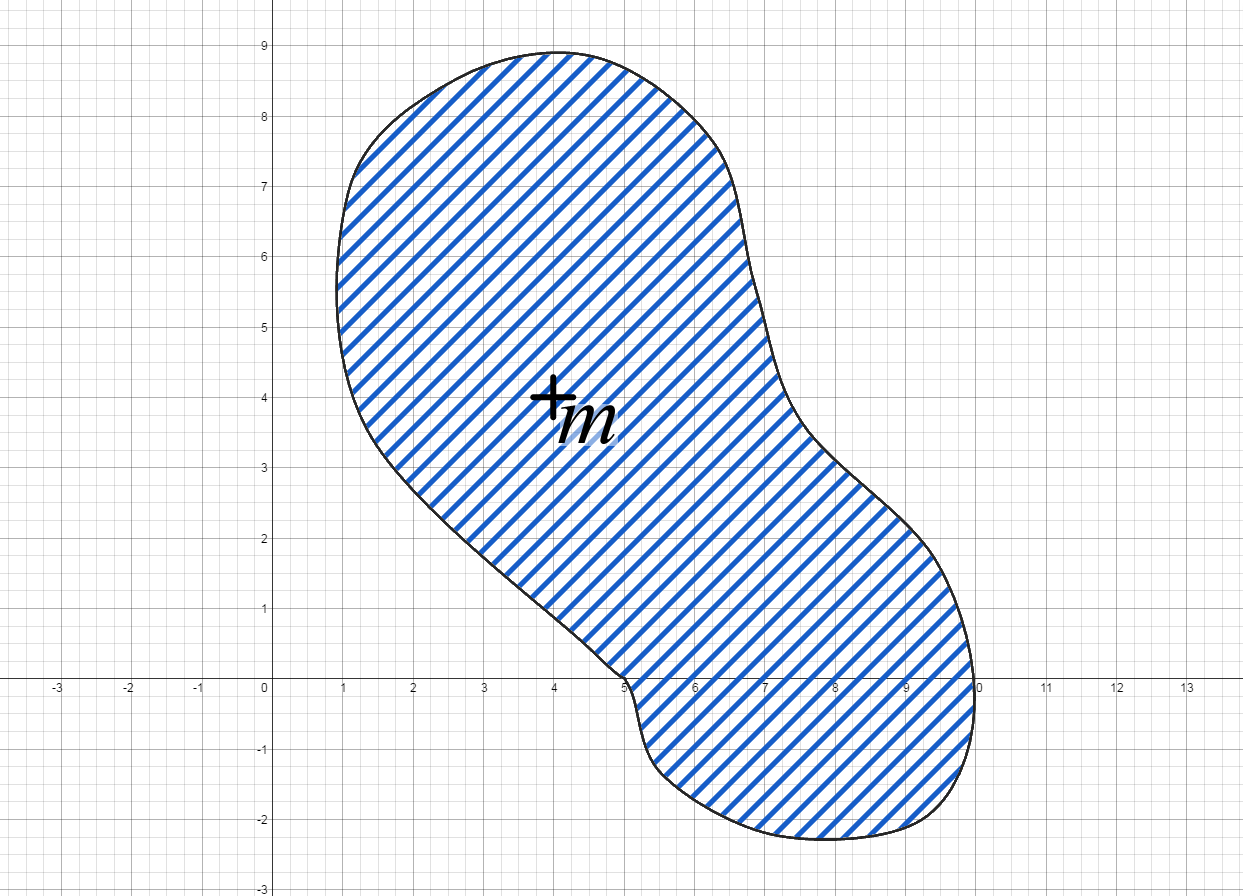
\includegraphics[width=\textwidth]{./potato-grid.png}
    \\
    \vspace{5mm} \hrule
    \newpage
    \section{The $ \textit{for-probably-all-} $quantifier}
    The \emph{for-probably-all}-quantifier (written as a \emph{W} combined with an vertically flipped \emph{A}) is a quantifier, which states that the given condition is \emph{probably} valid for all elements. The number of elements, for which the given condition is \emph{probably} valid must be a finite number.
    \\
    The following example demonstrates the use of the \emph{for-probably-all}-quantifier by assuming that one could divide by \emph{probably} every number in the field of rational numbers $ \mathbb{Q} $ :
    \begin{equation*}
        \begin{aligned}
            \fpa p,q \in \mathbb{Q} : pq^{-1} \in \mathbb{Q}
        \end{aligned}
    \end{equation*}
    As we very well know, one cannot divide a number by zero, thus the use of a \emph{for-all}-quantifier would be illegal. The \emph{for-probably-all}-quantifier, however, solves this problem, as the amount of elements whom which a number cannot be divided by (only zero) is finite:
    \begin{equation*}
        \begin{aligned}
            \{ q \in \mathbb{Q} \ | \ \verb"number cannot be divided by " q \}\sfa
        \end{aligned}
    \end{equation*}
    The formal definition for the \emph{for-probably-all}-quantifier is therefore:
    \begin{equation*}
        \begin{aligned}
            \text{let } M \subseteq \mathbb{K} \text{,} \quad \text{let } f : M \rightarrow \mathbb{B}
        \end{aligned}
    \end{equation*}
    \begin{equation*}
        \begin{aligned}
            \fpa k \in M : f(k)
            \quad :\Longleftrightarrow \quad
            \{ k \in M \ | \ \neg f(M) \}\sfa =: T \subsetneq \mathbb{K}
            \quad \wedge \quad
            \forall k \in M \backslash T : f(k)
        \end{aligned}
    \end{equation*}
    The \emph{for-probably-all}-quantifier can be seen as an implication of the \emph{for-all}-quantifier:
    \begin{equation*}
        \begin{aligned}
            \forall A \quad \Longrightarrow \quad \fpa A \qquad \qquad (A \in \mathbb{B})
        \end{aligned}
    \end{equation*}
    The probability, that the given statement $ A \in \mathbb{B} $ is probably true inside a \emph{for-all}-quantifier, when it has been proven true inside a \emph{for-probably-all}-quantifier, is called the \textit{magnitude of the for-probably-all-quantifier} and is usually written as $ \mathfrak{p} \in (0.5,1] $. \\ \\
    Example:
    \begin{equation*}
        \begin{aligned}
            \text{let } M = [-10, 10] \subseteq \mathbb{K} \text{,} \qquad \text{let } f : M \rightarrow \mathbb{B} : k \mapsto \exists^1 l \in M : k = -l
        \end{aligned}
    \end{equation*}
    \begin{equation*}
        \begin{aligned}
            \fpa k \in M : f(k) \quad \Longrightarrow \quad \mathfrak{p}(\forall k \in M : f(k)) > 99\%
        \end{aligned}
    \end{equation*}
    In the example above, the \emph{for-probably-all}-quantifier assumes, that with a probability of over 99\%, each element $ k \in M $ has an additive inverse element $ l \in M $, for which the equation $ k = -l $ is true.
    \\ \\
    Only with the use of highly sophisticated tools like \url{http://www.wolframalpha.com/}, one can decide whether the $ \forall $- or $ \exists^+ $-quantifier shall be used instead of the $ \fpa $-quantifier (hence also the symbol of the \emph{W} and \emph{A}, which can be interpreted as the initials of the name \emph{Wolfram|Alpha}).
    \vspace{5mm} \hrule
    \section{The $ \textit{troll} $-quantifier}
    The so-called \emph{troll}-quantifier is an variation of the \emph{exists}-quantifier, which states that the the given element usually exists .... \emph{but} one shall note, that it may also not exist:
    \begin{equation*}
        \begin{aligned}
            \text{let } M \subseteq \mathbb{K} \text{,} \qquad \text{let } f : M \rightarrow \mathbb{B}
        \end{aligned}
    \end{equation*}
    \begin{equation*}
        \begin{aligned}
            \bot k \in M : f(k) \quad :\Longleftrightarrow \quad \exists k \in M : f(k) \textcolor{gray}{\ \ ( \ \ \vee \ \ \ \nexists k \in M : f(k) \ \ )}
        \end{aligned}
    \end{equation*}
    The probability that the \emph{exists}-quantifier is true, when the \emph{troll}-quantifier has been proven true is called the \textit{magnitude of the troll-quantifier} and is usually written as $ \mathfrak{t} \in (0.5,1] $. The magnitudes $ \mathfrak{t} $ and  $ \mathfrak{p} $ are equal as shown as follows:
    \begin{equation*}
        \begin{aligned}
            \fpa A \ \Longrightarrow \ \bot A
            \qquad\qquad
            \mathfrak{p}(\forall A) \ =\ \mathfrak{t}(\exists A)
            \qquad\qquad
            (A \in \mathbb{B})
        \end{aligned}
    \end{equation*}
    The quantifiers can be ordered as follows (according to their implicity):
    \begin{equation*}
        \begin{aligned}
            \forall A \ \Longrightarrow \ \fpa A \ \Longrightarrow \ \exists^+ A \ \Longrightarrow \ \exists A \ \Longrightarrow \ \bot A
            \qquad\quad
            (A \in \mathbb{B})
        \end{aligned}
    \end{equation*}
    \vspace{5mm} \hrule
    \section{Polynomial final solution}
    A polynomial $ K \in \mathbb{K}[X] $ has a \emph{final solution} $ \mathcal{F}_x(K) $, if a graphic calculator yields the result \verb"10" (or sometimes \verb"9.5") after the polynomial has been typed. The procedure to find the \emph{final solution} $ \mathcal{F}(K) $ is unknown to mankind, yet some gifted mathematicians have found the way to calculate the \emph{final solution} $ \mathcal{F}_x(K) $ using a graphic calculator from the \textsc{Texas Instruments TI-83}-series. A possible procedure of solution could look as follows:
    \begin{equation*}
        \begin{aligned}
            \text{let } K \in \mathbb{K}[X] \text{,} \qquad \text{let } S \in \mathbb{K}
        \end{aligned}
    \end{equation*}
    \vbox{
        \vspace*{-25px}
        \begin{equation*}
            \begin{aligned}
                % \vspace*{-20px}
                \exists \mathcal{F}_x(K) = \langle 9.5 \ \ldots \ 10 \rangle \subsetneq \mathbb{K} \quad :\Longleftrightarrow \quad
                \exists S \in \raisebox{-20px}{ 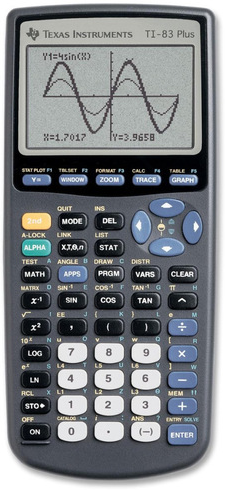
\includegraphics[height=40px]{./TI83.png} }(K) : \text{???}
            \end{aligned}
        \end{equation*}
    }
    \vspace{5mm} \hrule
    \section{The $ \emph{blah blah blah} $-operator}
    The so-called \emph{blah blah blah-operator} (also sometimes known as the \emph{dot-notation}) is a mathematical operator, which indicates the continuation of a previously given expression (modified by given contextual parameters). The following equations are examples for the usage of the \emph{blah blah blah-operator}:
    \begin{equation*}
        \begin{aligned}
            a_1 + a_2 + a_3 + \ldots \quad & :\Longleftrightarrow \quad \sum_{k=1}^{ \infty } b_{\substack{\\k}}
            \\
            f(x) = \langle sin, cos, -sin, -cos, \ldots \rangle (x) \quad & :\Longleftrightarrow \quad f(x) = \langle \ (sin(x))^{(n)}\ |\ n \in \mathbb{N}_0 \ \rangle
            \\
            \vdots \qquad \qquad & \qquad \qquad \vdots
        \end{aligned}
    \end{equation*}
    The \emph{blah blah blah-operator} may also be used inside a \emph{set-notation} as follows:
    \begin{equation*}
        \begin{aligned}
            [a \ldots b] \quad & :\Longleftrightarrow \quad \{ x \in \mathbb{K} | a \leq x \leq b : a,b \in \mathbb{K} \}
            \\
            [a_{\substack{\\k}}, a_{\substack{\\k+1}}, a_{\substack{\\k+2}}, \ldots] \quad & :\Longleftrightarrow \quad \{ a_i \in \mathbb{K} | i \geq k : i,k \in \mathbb{N}_0 \}
            \\
            \vdots \quad \quad & \qquad \qquad \qquad \vdots
        \end{aligned}
    \end{equation*}
    \vspace{5mm} \hrule
    \section{Unsort-sort}
    The \emph{unsort-sort} algorithm is a sorting algorithm, which uses a rather philosophical approach to array/list sorting:
    \newline
    The sorting algorithm is initialized with a ordered set $ S_0 \subseteq \mathbb{K} $, which will be defined as \textsc{ordered} list (independent from the 'real' value order of the list's elements). Any further given set $ S_n \subseteq \mathbb{K} $ will be sorted based on the given definition of \textsc{order}.
    \newline
    The \emph{unsort-sort} algorithm may be visualized by the following example:
    \begin{equation*}
        \begin{aligned}
            \text{let } \{3,1,5,4,2\} =: S_0 \subseteq \langle 1,5 \rangle =: K \subsetneq \mathbb{N} \text{ a ordered set and let }
            f : \mathcal{P}(\mathbb{K}) \mapsto \mathcal{P}(\mathbb{K}) \text{ be the sorting algorithm}
        \end{aligned}
    \end{equation*}
    \begin{equation*}
        \begin{aligned}
            \textsl{TODO}
            % \text{the set } \{1,2,3,4,5\} =: S_1 \subseteq K \text{ a ordered set}
        \end{aligned}
    \end{equation*}
    \vspace{5mm} \hrule
    \section{Interval constraints}
    A \emph{interval constraint} or \emph{set constraint} is usually applied to an interval- or range-notation and consists itself of a set, field or range. The constraint indicates that the target set is constructed only using the elements of the given constraint. e.g.:
    \begin{equation*}
        \begin{aligned}
            [1..5]_{\substack{\text{} \\ \mathbb{N}}} \ := \ \{1,2,3,4,5\} \ \neq \ \{1,2,0,1,2\} \ =: \ [1..5]_{\substack{\text{} \\ \mathbb{F}_3}}
        \end{aligned}
    \end{equation*}
    The formal definition of an \emph{interval/range/set/field constraint} is:
    \begin{equation*}
        \begin{aligned}
            & \text{let } \mathbb{K}_0 \text{ a field and } \mathcal{P}(\mathbb{K}_0) \ni K \subseteq \mathbb{K}_0 \text{ a subset of the field } \mathbb{K}_0
            \\
            & [a..b]_K \ = \ [a,b]_K \ := \ \{k \in K \ |\ a \leq k \leq b\} \qquad (a,b \in K, \ a \leq b)
            \\
            \\
            & \text{let } \mathbb{K}_1 \subseteq \mathbb{K}_0 \text{ be another field and } \mathcal{P}(\mathbb{K}_1) \ni L \subseteq \mathbb{K}_1 \text{ a subset of the field } \mathbb{K}_1
            \\
            & K_L \ := \ \{k \in K \ |\ k \in L\}\ = \ K \cap L \ \subseteq \ \mathbb{K}_0
        \end{aligned}
    \end{equation*}
    The the target set, range, interval or field must be a subset of the \emph{constraint}, rendering the following statement mathematically incorrect:
    \begin{equation*}
        \begin{aligned}
            (-6,-1]_{\substack{\text{} \\ \mathbb{N^+}}}
        \end{aligned}
    \end{equation*}
    \vspace{5mm} \hrule
    \section{<to be defined>}
    \textsl{<to be defined>}
\end{document}






% epsilon-zucchini
% wake on monog-drück-den power-knopf
% ip over praktikanten 